\documentclass{article}

\usepackage[ruled,vlined]{algorithm2e}
\usepackage[T1]{fontenc}
\usepackage[utf8]{inputenc}
\usepackage{amsmath}
\usepackage{amsfonts}
\usepackage{amssymb}
\usepackage{amsthm}
\usepackage{authblk}
\usepackage{graphicx}
\usepackage{hyperref}
\usepackage{lmodern}
\usepackage{microtype}
\usepackage{subcaption}

\usepackage{graphicx}
\graphicspath{ {img/} }

\usepackage[backend=biber,style=authoryear-comp]{biblatex}
\addbibresource{references.bib}

\title{Generating Synthetic Financial Time-Series Data Through Generative Adversatial Network\\[0.5em] \large Methodologies And Comparison Among Different Deep Learning Structures}

\author[1]{Grant Sawyer\thanks{\href{mailto:gsawyer@andrew.cmu.edu}{gsawyer@andrew.cmu.edu}}}
\author[1]{Harold Yuan\thanks{\href{mailto:zhongfay@andrew.cmu.edu}{zhongfay@andrew.cmu.edu}}}
\author[1]{Kaushik Tallam\thanks{\href{mailto:ktallam@andrew.cmu.edu}{ktallam@andrew.cmu.edu}}}
\author[1]{Mario Nicolo' De Matteis\thanks{\href{mailto:mdematte@andrew.cmu.edu}{mdematte@andrew.cmu.edu}}}
\author[1]{Tristan Roemer\thanks{\href{mailto:troemer@andrew.cmu.edu}{troemer@andrew.cmu.edu}}}

\affil[1]{Carnegie Mellon University, MSCF, New York, USA}

\usepackage{cleveref}
\usepackage{geometry}
\geometry{a4paper, margin=1in}

\date{February 2025}

\begin{document}

\maketitle

\begin{abstract}
    Generative Adversarial Networks (GANs) have emerged as a powerful tool for synthesizing realistic financial time-series data, addressing challenges such as data scarcity, privacy, and cost. This paper explores the integration of attention mechanisms, convolutional neural networks (CNNs), and long short-term memory (LSTM) layers within a GAN framework to generate synthetic financial price data. We evaluate the performance of these architectures using three financial instruments—JPMorgan Chase (JPM), Apple Inc. (AAPL), and the MSCI ACWI Index (ACWI)—spanning over two decades of market data. Our results demonstrate that CNN-enhanced GANs significantly improve the modeling of temporal dependencies and volatility clustering compared to Attention- and LSTM-based variants. The synthetic data exhibits statistical properties closely aligned with real-world financial time series, as validated by rigorous tests for distributional similarity and moments. These findings provide actionable insights for financial institutions seeking to augment datasets for backtesting, risk management, and machine learning applications.
\end{abstract}

\noindent \textbf{Keywords:} Generative Adversatial Networks, Financial Time-Series, Attention Layers

\section{Introduction}

Hedge Funds, Proprietary Trading Firms, and other financial institutions rely on large amounts of data to make informed decisions. However, obtaining high-quality financial data can be challenging due to privacy concerns, data access restrictions, and the high cost of data acquisition. To address these challenges, researchers have developed generative models that can synthesize realistic financial time-series data. These models can be used to augment existing datasets, generate new data for backtesting trading strategies, and simulate market conditions for risk management. Over the last few years, many different developments have been conducted in the field of synthethic financial time-series data generation. In this paper, we provide a comprehensive overview of the methodologies and comparison among different deep learning structures used to generate synthetic financial time-series data. In particular, we aim to synthesize new price time series data that can be highly useful for various applications. These include backtesting trading strategies, training machine learning models, and conducting stress tests and scenario analyses. By generating realistic synthetic data, we can provide financial institutions with a valuable resource to enhance their decision-making processes, improve model robustness, and better prepare for adverse market conditions.

Given the great impact and power of generative AI models, we decided to exploit one of the main pillars of Generative AI: the Generative Adversarial Network develope by \textcite{goodfellow_generative_2014}. GANs have been extensively used in the computer vision field, particularly in image generation. \textcite{iglesias_survey_2023} show the ability to generate realistic data samples through adversarial training makes them a powerful tool for synthesizing financial time-series data as well. This groundbreaking model has profoundly influenced subsequent research by demonstrating that adversarial training can generate remarkably realistic data samples. \textcite{EckerliFlorian2021GANi} mentions different applications of GANs, including market manipulation, credit card fraud, portfolio optimization and market prediction.

In the realm of synthetic financial data, several other aspects are equally important. For example, robust data augmentation techniques can enhance model reliability, and careful evaluation of synthetic data against real-world financial indicators is crucial for ensuring its practical utility. Moreover, addressing the temporal dependencies and non-linear dynamics inherent in financial markets requires advanced modeling techniques that go beyond the original GAN framework. In simple terms, we aim to find out the distribution by which the prices have been generated. When looking for new data, among the most well-known techniques, we recall different and exotic sampling techniques that tend to be very complex and computationally expensive. As highlighted by \textcite{cont_empirical_2001}, understanding the empirical properties of asset returns, such as heavy tails and volatility clustering, is essential for developing realistic financial models. These properties must be carefully considered when designing synthetic data generation frameworks to ensure that the generated data accurately reflects the behavior observed in real financial markets.

We designed the neural networks for the GAN models by implementing three different types of layers: Attention, CNN, and LSTM. We decided to implement these three different types of layers because each offers unique advantages for capturing the complex dynamics of financial time series data. In accordance with the literature, Attention layers allow the model to focus on significant temporal patterns, enhancing its ability to prioritize key segments of the data. Convolutional Neural Networks (CNNs) are effective at detecting localized patterns and extracting spatial features, which are crucial for modeling short-term trends and volatility clusters. Long Short-Term Memory (LSTM) networks excel at capturing long-range dependencies and the sequential nature of financial data, making them ideal for modeling the temporal evolution of asset prices. By integrating these diverse neural network components, we aim to improve the overall performance and robustness of our GAN models in generating realistic synthetic financial time series data.

Building on these insights, our paper aims to explore and compare the effectiveness of various neural network architectures within the GAN framework. In particular, we focus on:
\begin{itemize}
    \item \textbf{Attention Layers}: To capture and prioritize significant temporal patterns, thereby enabling the model to focus on key segments of the time series.
    \item \textbf{Convolutional Neural Networks (CNNs)}: To detect localized patterns and extract spatial features from financial time series data.
    \item \textbf{Long Short-Term Memory (LSTM) Networks}: To model long-range dependencies and effectively capture the sequential characteristics of financial data.
\end{itemize}

Through a detailed comparative analysis, this study evaluates the performance of these architectures in generating synthetic financial time series data. In particular, we investigate how the integration of attention mechanisms can enhance the synthesis process by more accurately reflecting the intricate dynamics of financial markets.

\vspace{1em}
\noindent\textit{The project code, datasets, and additional resources are available at our GitHub repository: \url{https://github.com/mariodematteis/ml-ii-final-project}.}

\section{Data and Variables of Interest}

In this study, we focus on synthesizing financial time series data using a Generative Adversarial Network (GAN) framework. The selection of financial instruments is a critical component in ensuring that our model is both robust and generalizable. To this end, we have chosen three key instruments: JPMorgan Chase (JPM), Apple Inc. (AAPL), and the MSCI ACWI Index (ACWI). These selections enable us to assess our model's performance across both individual equities and a broad market index, which together represent a wide array of market dynamics.

Data for these financial instruments was sourced from the Wharton Research Data Services (WRDS) platform, which provides extensive access to high-quality daily historical data. For JPM and AAPL, the dataset spans from January 1, 2000, to January 31, 2024. This period covers multiple market cycles and includes significant economic events, thereby offering a rich context for capturing the complex dynamics inherent in financial markets. Such an extensive historical record is invaluable for training deep learning models, as it encompasses both periods of high volatility and relative stability.

In contrast, the historical data for the MSCI ACWI index is available from March 28, 2008 onward. Although this dataset has a shorter temporal coverage compared to the individual stock data, the ACWI index represents a diversified portfolio of global equities, including both developed and emerging markets. This diversification is instrumental in evaluating the generalizability of the synthetic data generated by our model across different market conditions and geographic regions.

The integration of these datasets ensures a comprehensive evaluation of our GAN-based approach. In subsequent sections, we describe the preprocessing steps applied to the raw data, including cleaning, normalization, and the transformation procedures that were necessary to render the data suitable for model training. This careful curation and preparation of the dataset lay the groundwork for the subsequent analysis of model performance, particularly with respect to the incorporation of Attention layers, Convolutional Neural Networks, and Long Short-Term Memory (LSTM) networks.

\section{Model}

Generative Adversarial Networks (GANs) provide a framework to learn complex data distributions through a two-player minimax game involving two neural networks: a \textbf{generator} and a \textbf{discriminator}. The classical formulation of GANs is outlined below, after which we describe our enhanced generator architectures that incorporate attention, convolutional, and long short-term memory layers.

\subsection*{1. Setup and Notation}

\begin{itemize}
    \item \textbf{Real Data Distribution:} Let $p_{\text{data}}(x)$ denote the probability distribution of real data samples $x \in \mathcal{X}$.
    \item \textbf{Latent Space and Prior:} Define a latent space $\mathcal{Z}$ with a simple prior distribution $p_z(z)$ (e.g., a Gaussian or uniform distribution). A latent variable $z \sim p_z(z)$ is sampled and then transformed into the data space.
    \item \textbf{Generator:} The generator is a function $G: \mathcal{Z} \to \mathcal{X}$ parameterized by $\theta_G$. It maps a latent variable $z$ to a synthetic sample $G(z)$, thereby inducing an implicit distribution $p_g(x)$ over the data space.
    \item \textbf{Discriminator:} The discriminator is a function $D: \mathcal{X} \to [0,1]$ parameterized by $\theta_D$. It outputs a scalar representing the probability that a given sample $x$ originates from the real data distribution $p_{\text{data}}(x)$ rather than from $p_g(x)$.
\end{itemize}

\subsection*{2. The Minimax Game}

The GAN framework is formulated as a two-player minimax game with the value function

\[
\min_{G} \max_{D} V(D,G) = \mathbb{E}_{x\sim p_{\text{data}}(x)}\big[\log D(x)\big] + \mathbb{E}_{z\sim p_z(z)}\big[\log (1 - D(G(z)))\big].
\]

\begin{itemize}
    \item \textbf{Discriminator’s Objective:} For a fixed generator $G$, the discriminator $D$ is trained to maximize the probability of correctly classifying real data and generated data:

    \[
    \mathbb{E}_{x\sim p_{\text{data}}(x)}\big[\log D(x)\big] + \mathbb{E}_{x\sim p_g(x)}\big[\log (1 - D(x))\big].
    \]

    \item \textbf{Generator’s Objective:} Simultaneously, the generator $G$ is trained to minimize the same objective (i.e., to “fool” $D$) by generating samples $G(z)$ that maximize the discriminator's misclassification:

    \[
    \min_{G} \mathbb{E}_{z\sim p_z(z)}\big[\log (1 - D(G(z)))\big].
    \]
\end{itemize}

\subsection*{3. Optimal Discriminator and Jensen-Shannon Divergence}

For any fixed generator $G$, the optimal discriminator $D^*_G(x)$ is obtained by maximizing the value function pointwise:
\[
f(D(x)) = p_{\text{data}}(x) \log D(x) + p_g(x) \log (1 - D(x)).
\]
Taking the derivative with respect to $D(x)$ and setting it to zero leads to:
\[
\frac{p_{\text{data}}(x)}{D(x)} - \frac{p_g(x)}{1-D(x)} = 0 \quad \Longrightarrow \quad D^*_G(x) = \frac{p_{\text{data}}(x)}{p_{\text{data}}(x) + p_g(x)}.
\]
Substituting $D^*_G$ back into the value function yields:
\[
V(G, D^*_G) = -\log(4) + 2\, \mathrm{JSD}\big(p_{\text{data}} \,\|\, p_g\big),
\]
where $\mathrm{JSD}$ denotes the Jensen-Shannon Divergence. Minimizing $V(G, D^*_G)$ with respect to $G$ forces $p_g(x)$ to converge to $p_{\text{data}}(x)$.

\subsection*{4. Training Procedure}

In practice, GAN training alternates between:
\begin{enumerate}
    \item \textbf{Discriminator Update:} Maximize $V(D, G)$ with respect to $\theta_D$, keeping $\theta_G$ fixed.
    \item \textbf{Generator Update:} Minimize $V(D, G)$ (or a modified loss, such as maximizing $\log D(G(z))$ for stronger gradients) with respect to $\theta_G$, while keeping $\theta_D$ fixed.
\end{enumerate}
These updates are typically performed using stochastic gradient descent or its variants.

\subsection*{5. Enhanced Generator Architectures}

While the classical GAN framework provides a robust foundation for generative modeling, financial time series data pose unique challenges due to their complex temporal dependencies and non-linear structures. To address these issues, we extend the generator architecture by incorporating advanced neural network components, as detailed below.

\subsubsection*{5.1 Attention Layers}

Attention mechanisms enable the model to dynamically focus on different parts of the input sequence, assigning higher weights to temporally significant features. Inspired by the Transformer architecture, our attention layer computes a weighted sum of feature representations across time steps. This mechanism is crucial for capturing long-range dependencies and subtle patterns that might be missed by standard sequential models. The attention layer is integrated into the generator to selectively emphasize critical time steps during the generation process.

\subsubsection*{5.2 Convolutional Neural Networks (CNNs)}

Convolutional layers are effective at extracting localized features and detecting patterns within data. In the context of financial time series, CNNs can capture short-term trends and volatility clusters by applying convolutional filters along the temporal dimension. These filters learn hierarchical representations, which are instrumental in modeling the non-stationary characteristics of asset prices. Previous studies have shown the efficacy of CNNs in time series forecasting and anomaly detection. In our generator, convolutional layers are employed to extract spatial-temporal features before the data is processed by other sequential layers.

\subsubsection*{5.3 Long Short-Term Memory (LSTM) Networks}

LSTM networks are a natural choice for modeling sequential data due to their ability to capture long-term dependencies and mitigate issues such as vanishing gradients. The gating mechanisms in LSTMs allow the network to remember relevant information over extended periods, which is essential for accurately modeling the evolution of financial time series. LSTMs have been widely used in various forecasting tasks and have proven effective in capturing both short-term fluctuations and long-term trends . In our framework, LSTM layers are used to process the sequential output from convolutional layers or attention modules, further refining the temporal dynamics captured in the generated data.

\subsubsection*{5.4 Integration within the GAN Framework}

In our proposed model, these enhanced architectural components are integrated within the generator network while the discriminator maintains a conventional architecture. This integration is designed to evaluate the impact of each component on the quality of the generated synthetic financial time series. The overall training procedure remains consistent with the classical GAN paradigm, with the generator updates now encompassing additional hyperparameters related to the attention heads, convolutional filter sizes, and LSTM layer configurations.

By comparing these variants, our study aims to elucidate the advantages and limitations of incorporating attention mechanisms, CNNs, and LSTMs in the context of synthetic financial data generation. The experimental evaluation (detailed in Section ) provides insights into how these components improve the generator's ability to model the intricate, non-linear, and temporal structures present in real financial time series.

\section{Results and Evaluations}

By taking a look at the appendix, it is possible to observe that among the three different implementation, the one based on the convolutional performs better in terms of returns distribution. Visually, the log returns of the generated data look very similar to the log returns of the historical data. It is possible to analyze this result also from a more statitical perspective like the Jensen-Shannon divergence. The model based on the convolutional layers shows best results for Apple and the MSCI ACWI Index, however, does not adequately capture the market dynamics for JP Morgan, whose generated returns look to be more volatile compared to the ones coming from the historical data.

For CNN, looking at the Jensen-Shannon Divergence (JSD, min. of 0 and max. of $ ln(2) = 0.693 $) we get a score in the order of $ 10^{-1} $ which is very good. JPM on the otherhand is quite high with a score of 0.251. We see that the generated distribution has considerably fatter tails, especially a fatter left tail which would explain why all the generated time series plotted above for JPM have a drastic negative spike at one location. This may have been caused by a large drawdown during a short time period in the historical data that the model overemphasized during training, or perhaps a data error. The LSTM model performs worst according to JSD and produces a much too narrow distribution, which may indicate that there was some sort of structural mistake in applying that architecture to our data. Perhaps after tuning the architecture for our data better and retraining we would achieve better results. The attention model manages to produce better distributions than the LSTM, however, they are also not very strongly aligned with historical data. Specifically for ACWI, the Attention architecture does quite okay (visually) with a JSD of 0.222. Overall, both visually and numerically, the CNN GAN strongly outcompetes the other specific architectures used in this paper in generating synthetic time series.

It is also interesting to look at autocorrelation for our time series which is another important metric of market dynamics. In our historical data, JPM and ACWI showed evidence of autocorrelation, while AAPL did not, as seen by the Ljung-Box tests in the tables in the appendix. Our generated data showed autocorrelation for all 3 tickers in all 3 models. Which means that it either correctly generates autocorrelated data for 2/3 tickers, or, the architecture and methodology potentially always generates autocorrelated data.

\section{Conclusion}

In conclusion, our investigation into enhanced GAN architectures for synthesizing financial time series data demonstrates that incorporating convolutional layers yields superior performance in capturing the distributional characteristics of asset returns compared to LSTM and attention-based models. While the CNN-based model successfully replicates the historical return distributions for instruments such as AAPL and the MSCI ACWI Index, discrepancies observed for JPM highlight areas for further refinement. Future work should explore additional tuning of the architectures and consider hybrid approaches that combine the strengths of attention, CNNs, and LSTMs to achieve even closer alignment with real market data. These improvements could provide financial institutions with more robust synthetic datasets for applications in backtesting, risk management, and machine learning research.

\section*{Acknowledgments}

We would like to thank CodeWilling for providing the computational resources that enabled us to train and evaluate our models effectively.

\printbibliography

\appendix
\section{Appendix}

\begin{table}[ht]
\centering
\begin{tabular}{lcc}
\hline
\textbf{Metric} & \textbf{Original} & \textbf{Generated} \\
\hline
Mean     & 0.000128 & -0.000002 \\
Std      & 0.040645 & 0.214407 \\
Skewness & -25.111799 & 0.255764 \\
Kurtosis & 1039.042700 & 46.728140 \\
Ljung-Box t-statistic & 10.673040 & 272346.309774 \\
Ljung-Box p-value & 0.383552 & 0.000000 \\
\hline
\end{tabular}
\caption{AAPL Moments Comparison for the Attention-Based GAN.
Jensen--Shannon Divergence: 0.580034}
\label{tab:aapl_attention}
\end{table}

\begin{table}[ht]
\centering
\begin{tabular}{lcc}
\hline
\textbf{Metric} & \textbf{Original} & \textbf{Generated} \\
\hline
Mean     & 0.000279 & 0.000001 \\
Std      & 0.012906 & 0.079548 \\
Skewness & -0.556542 & -0.786310 \\
Kurtosis & 11.866263 & 135.567522 \\
Ljung-Box t-statistic & 55.307795 & 1234.989861 \\
Ljung-Box p-value & 0.000000 & 0.000000 \\
\hline
\end{tabular}
\caption{ACWI Moments Comparison for the Attention-Based GAN.
Jensen--Shannon Divergence: 0.221720}
\label{tab:acwi_attention}
\end{table}

\begin{table}[ht]
\centering
\begin{tabular}{lcc}
\hline
\textbf{Metric} & \textbf{Original} & \textbf{Generated} \\
\hline
Mean     & 0.000189 & -0.000002 \\
Std      & 0.104471 & 0.198215 \\
Skewness & -0.021890 & 0.098549 \\
Kurtosis & 106.470019 & 30.823050 \\
Ljung-Box t-statistic & 1442.181508 & 247959.786055 \\
Ljung-Box p-value & 0.000000 & 0.000000 \\
\hline
\end{tabular}
\caption{JPM Moments Comparison for the Attention-Based GAN.
Jensen--Shannon Divergence: 0.504067}
\label{tab:jpm_attention}
\end{table}

\begin{table}[h!]
\centering
\begin{tabular}{lcc}
\hline
\textbf{Metric} & \textbf{Original} & \textbf{Generated} \\
\hline
Mean     & 0.000128 & 0.000003 \\
Std      & 0.040645 & 0.180111 \\
Skewness & -25.111799 & -0.640448 \\
Kurtosis & 1039.042700 & 158.044933 \\
Ljung-Box t-statistic & 10.673040 & 347.086390 \\
Ljung-Box p-value & 0.383552 & 0.000000 \\
\hline
\end{tabular}
\caption{AAPL Moments Comparison for the CNN-Based GAN.
Jensen--Shannon Divergence: 0.060796}
\label{tab:aapl_cnn}
\end{table}

\begin{table}[h!]
\centering
\begin{tabular}{lcc}
\hline
\textbf{Metric} & \textbf{Original} & \textbf{Generated} \\
\hline
Mean     & 0.000279 & -0.000001 \\
Std      & 0.012906 & 0.082028 \\
Skewness & -0.556542 & -0.880490 \\
Kurtosis & 11.866263 & 143.158931 \\
Ljung-Box t-statistic & 55.307795 & 264.902105 \\
Ljung-Box p-value & 0.000000 & 0.000000 \\
\hline
\end{tabular}
\caption{ACWI Moments Comparison for the CNN-Based GAN.
Jensen--Shannon Divergence: 0.065261}
\label{tab:acwi_cnn}
\end{table}

\begin{table}[h!]
\centering
\begin{tabular}{lcc}
\hline
\textbf{Metric} & \textbf{Original} & \textbf{Generated} \\
\hline
Mean     & 0.000189 & -0.000001 \\
Std      & 0.104471 & 0.174060 \\
Skewness & -0.021890 & 1.247102 \\
Kurtosis & 106.470019 & 60.163179 \\
Ljung-Box t-statistic & 1442.181508 & 64169.776953 \\
Ljung-Box p-value & 0.000000 & 0.000000 \\
\hline
\end{tabular}
\caption{JPM Moments Comparison for the CNN-Based GAN.
Jensen--Shannon Divergence: 0.251107}
\label{tab:jpm_cnn}
\end{table}

\begin{table}[h!]
\centering
\begin{tabular}{lcc}
\hline
\textbf{Metric} & \textbf{Original} & \textbf{Generated} \\
\hline
Mean     & 0.000128 & -0.000005 \\
Std      & 0.040645 & 0.168739 \\
Skewness & -25.111799 & 0.647168 \\
Kurtosis & 1039.042700 & 150.256361 \\
Ljung-Box t-statistic & 10.673040 & 1412.511109 \\
Ljung-Box p-value & 0.383552 & 0.000000 \\
\hline
\end{tabular}
\caption{AAPL Moments Comparison for the LSTM-Based GAN.
Jensen--Shannon Divergence: 0.608428}
\label{tab:aapl_attention}
\end{table}

\begin{table}[h!]
\centering
\begin{tabular}{lcc}
\hline
\textbf{Metric} & \textbf{Original} & \textbf{Generated} \\
\hline
Mean     & 0.000279 & -0.000000 \\
Std      & 0.012906 & 0.084201 \\
Skewness & -0.556542 & 2.924553 \\
Kurtosis & 11.866263 & 80.666600 \\
Ljung-Box t-statistic & 55.307795 & 3032.228573 \\
Ljung-Box p-value & 0.000000 & 0.000000 \\
\hline
\end{tabular}
\caption{ACWI Moments Comparison for the LSTM-Based GAN.
Jensen--Shannon Divergence: 0.601836}
\label{tab:acwi_lstm}
\end{table}

\begin{table}[h!]
\centering
\begin{tabular}{lcc}
\hline
\textbf{Metric} & \textbf{Original} & \textbf{Generated} \\
\hline
Mean     & 0.000189 & 0.000002 \\
Std      & 0.104471 & 0.120360 \\
Skewness & -0.021890 & -0.977749 \\
Kurtosis & 106.470019 & 132.980503 \\
Ljung-Box t-statistic & 1442.181508 & 6376.462484 \\
Ljung-Box p-value & 0.000000 & 0.000000 \\
\hline
\end{tabular}
\caption{JPM Moments Comparison for the LSTM-Based GAN.
Jensen--Shannon Divergence: 0.596089}
\label{tab:jpm_lstm}
\end{table}

\begin{figure}[h!]
    \centering
    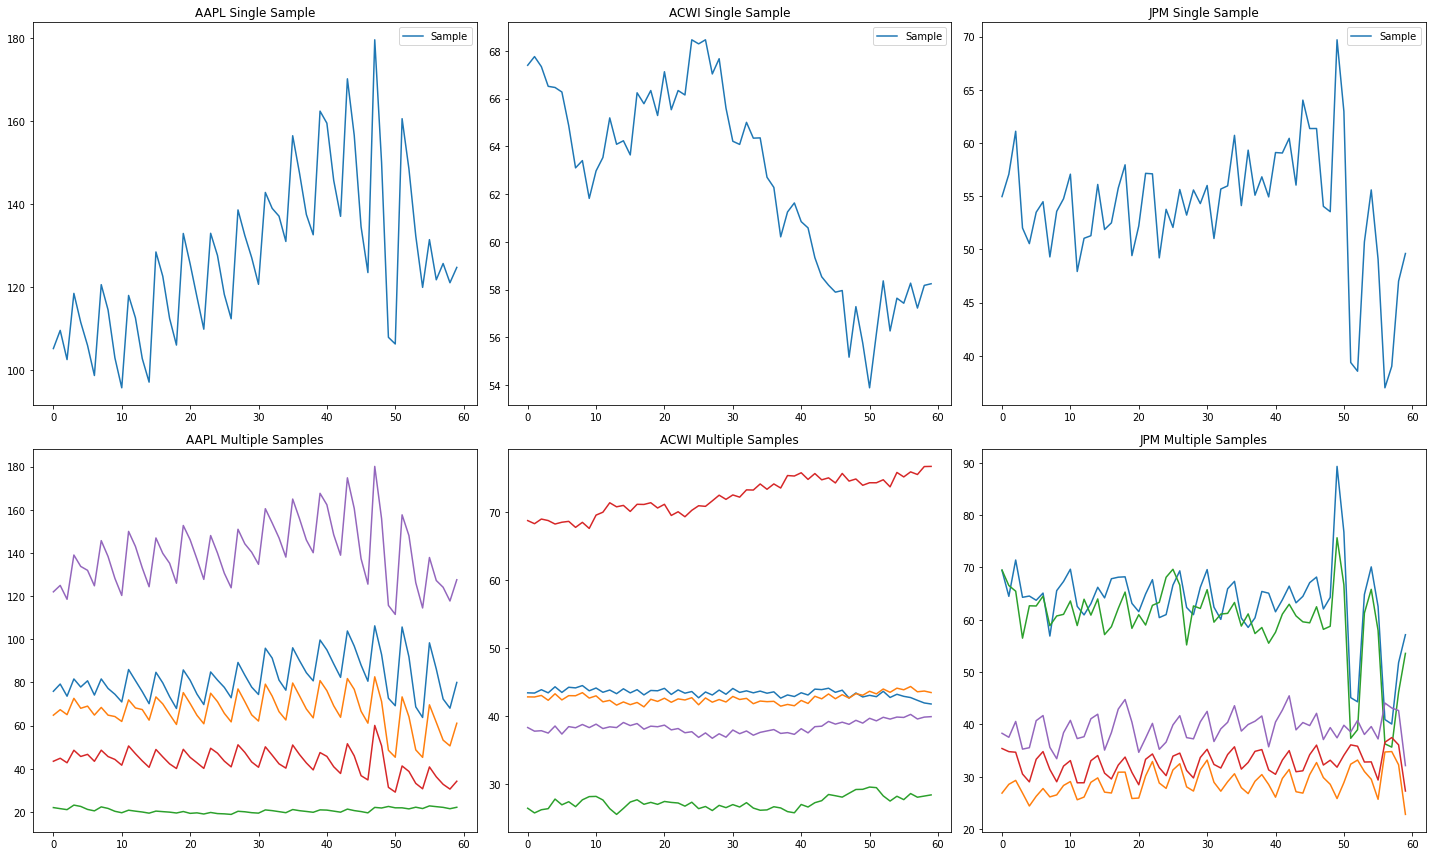
\includegraphics[width=0.7\textwidth]{attention_gen_samples}
    \caption{Comparison of Real vs. Generated Time Series for AAPL, ACWI and JPM using Attention-Based GAN.}
    \label{fig:attention_comparison}
\end{figure}

\begin{figure}[h!]
    \centering
    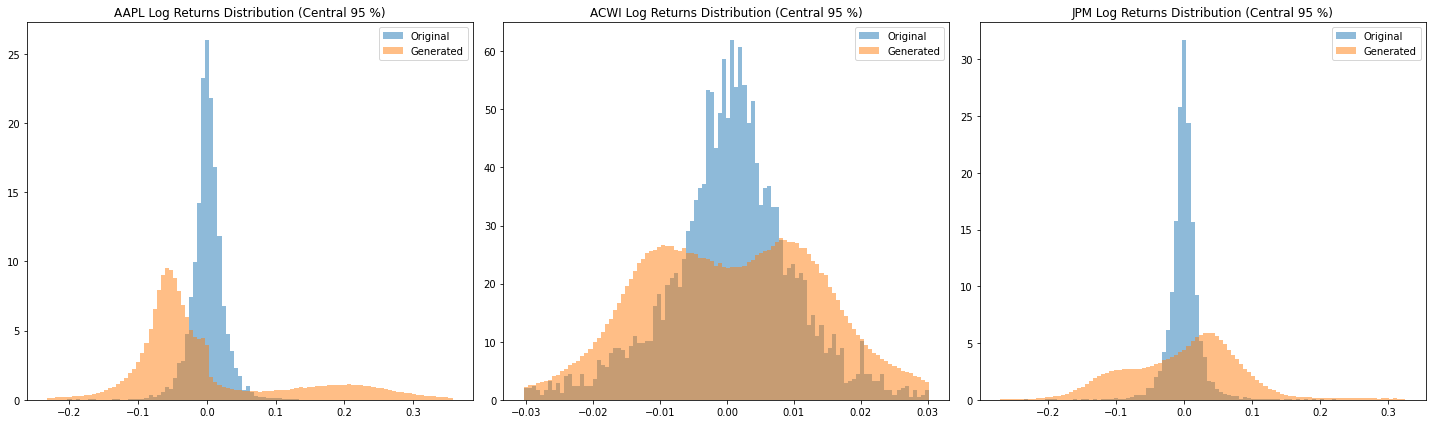
\includegraphics[width=0.7\textwidth]{attention_distributions}
    \caption{Comparison of Real vs. Generated Log-Return Distributions for AAPL, ACWI and JPM using Attention-Based GAN.}
    \label{fig:attention_comparison}
\end{figure}

\begin{figure}[h!]
    \centering
    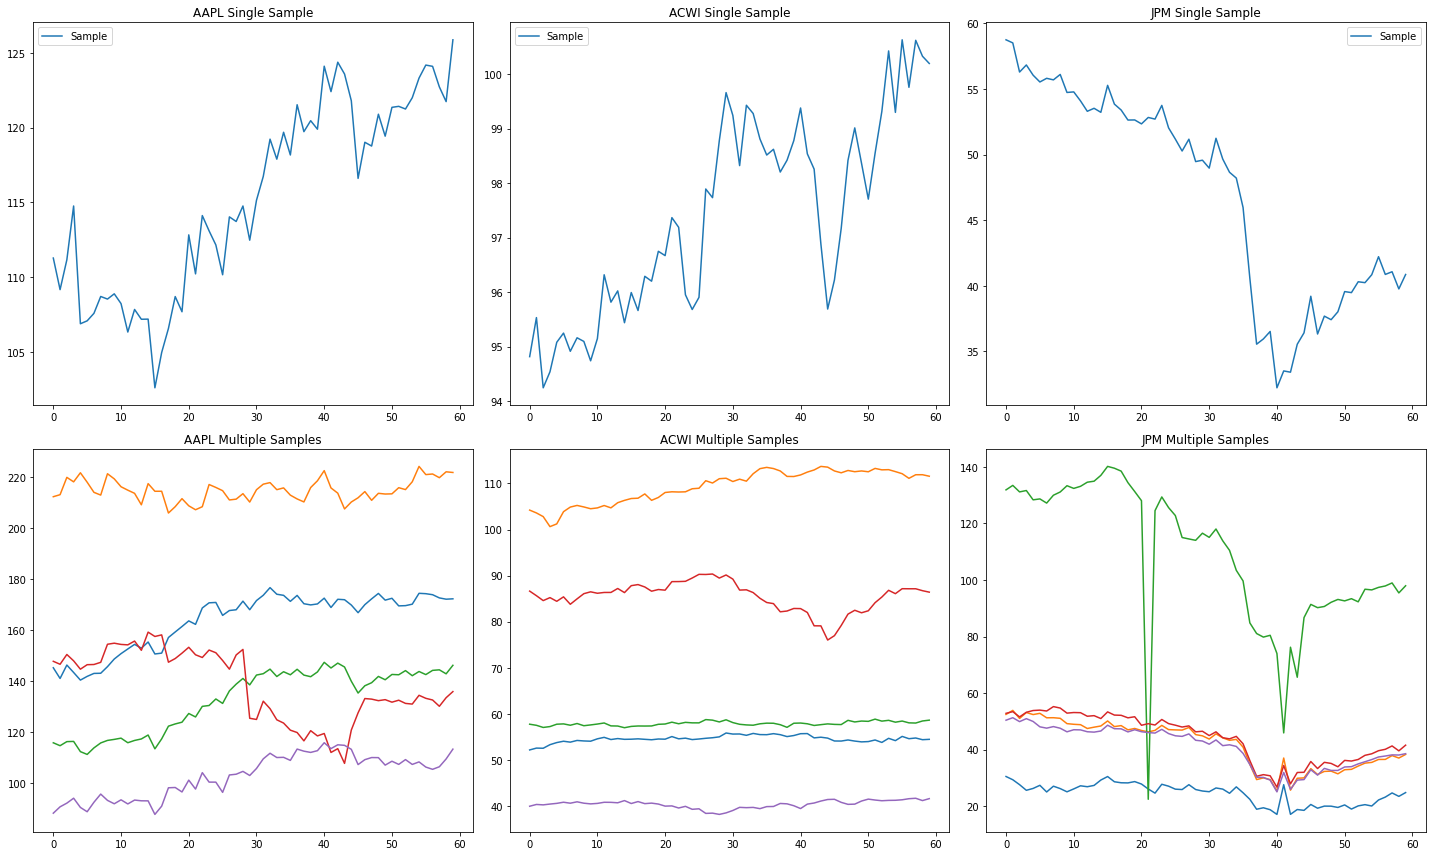
\includegraphics[width=0.7\textwidth]{CNN_gen_samples}
    \caption{Comparison of Real vs. Generated Time Series for AAPL, ACWI and JPM using Attention-Based GAN.}
    \label{fig:attention_comparison}
\end{figure}

\begin{figure}[h!]
    \centering
    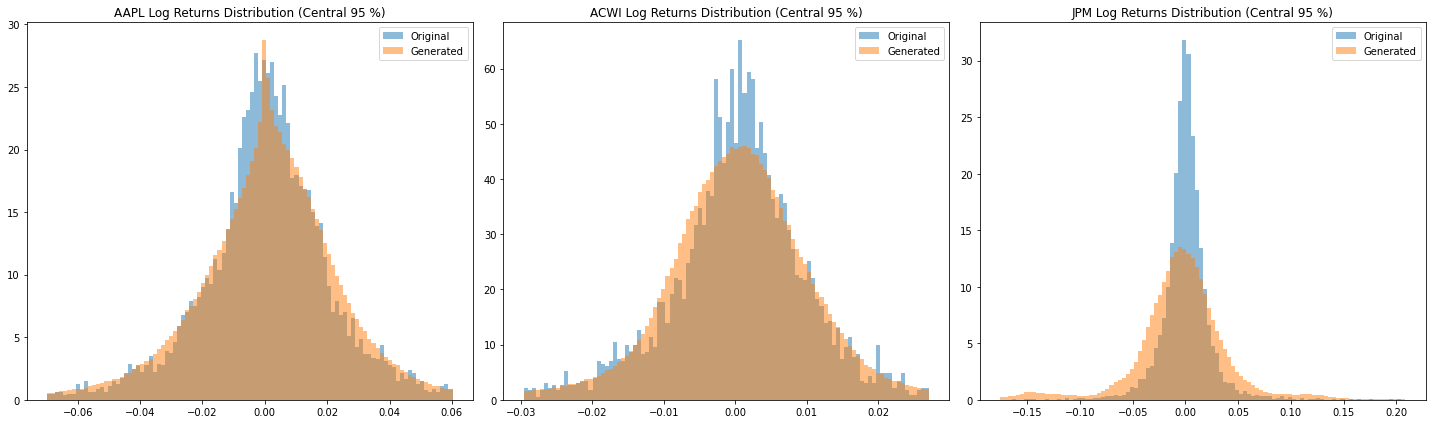
\includegraphics[width=0.7\textwidth]{cnn_distributions}
    \caption{Comparison of Real vs. Generated Log-Return Distributions for AAPL, ACWI and JPM using CNN-Based GAN.}
    \label{fig:attention_comparison}
\end{figure}

\begin{figure}[h!]
    \centering
    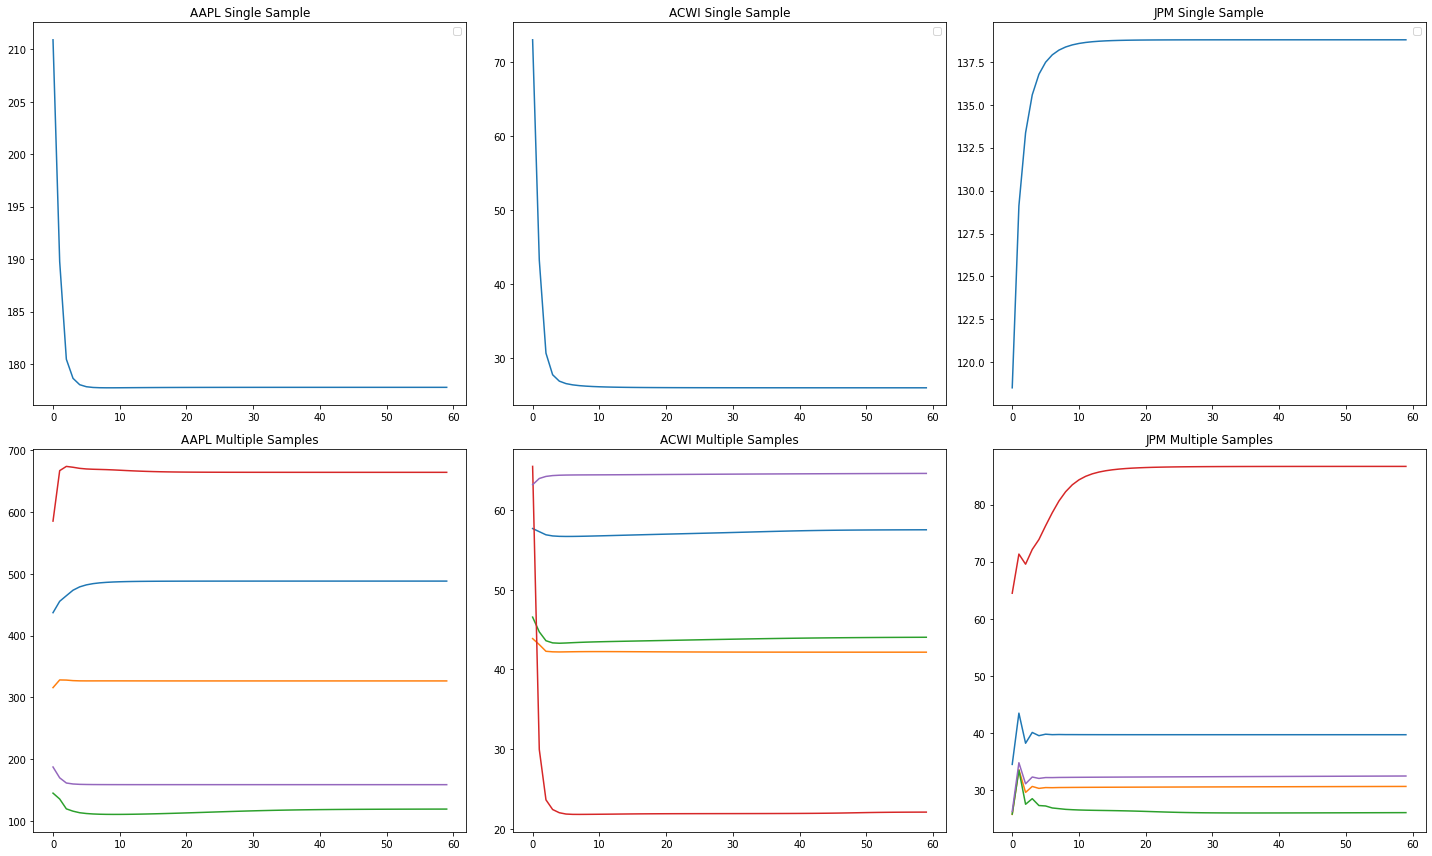
\includegraphics[width=0.7\textwidth]{LSTM_gen_samples}
    \caption{Comparison of Real vs. Generated Time Series for AAPL, ACWI and JPM using LSTM-Based GAN.}
    \label{fig:attention_comparison}
\end{figure}

\begin{figure}[h!]
    \centering
    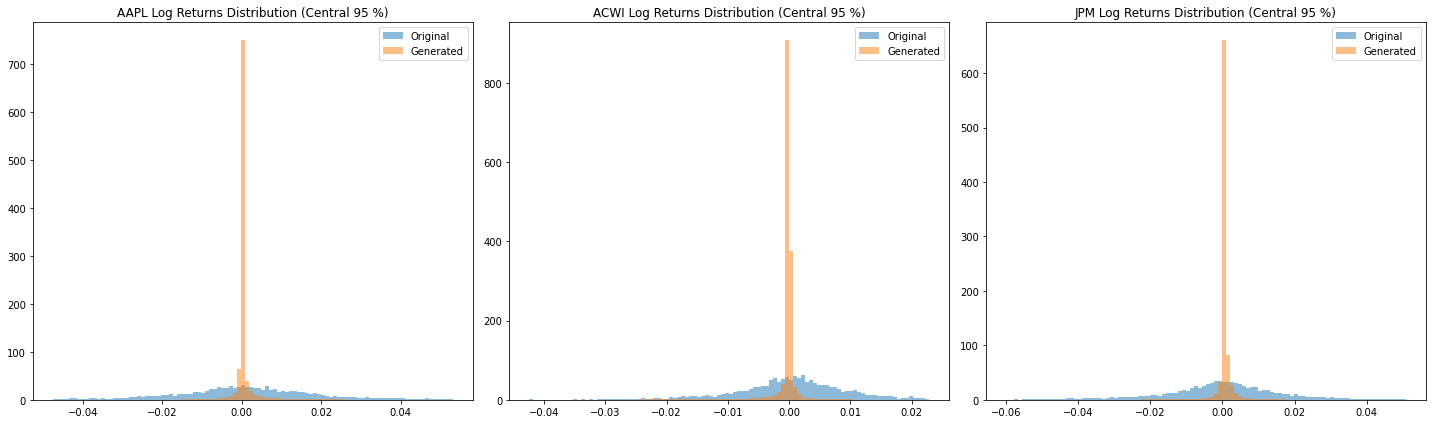
\includegraphics[width=0.7\textwidth]{LSTM_distributions}
    \caption{Comparison of Real vs. Generated Log-Return Distributions for AAPL, ACWI and JPM using LSTM-Based GAN.}
    \label{fig:attention_comparison}
\end{figure}

\end{document}
